\documentclass[aps,prb,twocolumn,superscriptaddress,floatfix,longbibliography]{revtex4-2}

\usepackage[utf8]{inputenc}
\usepackage[spanish]{babel}
\usepackage{graphicx}
\usepackage{amsmath}
\usepackage{subcaption}
\usepackage{wrapfig} 
\usepackage[export]{adjustbox}

\usepackage{amsmath,amssymb} % math symbols
\usepackage{bm} % bold math font
\usepackage{graphicx} % for figures
\usepackage{comment} % allows block comments
\usepackage{textcomp} % This package is just to give the text quote '
%\usepackage{ulem} % allows strikeout text, e.g. \sout{text}

\usepackage[spanish]{babel}

\usepackage{enumitem}
\setlist{noitemsep,leftmargin=*,topsep=0pt,parsep=0pt}

\usepackage{xcolor} % \textcolor{red}{text} will be red for notes
\definecolor{lightgray}{gray}{0.6}
\definecolor{medgray}{gray}{0.4}

%Para las tablas
\usepackage{multirow}

\usepackage{hyperref}
\hypersetup{
colorlinks=true,
urlcolor= blue,
citecolor=blue,
linkcolor= blue,
bookmarks=true,
bookmarksopen=false,
}

% Code to add paragraph numbers and titles
\newif\ifptitle
\newif\ifpnumber
\newcounter{para}
\newcommand\ptitle[1]{\par\refstepcounter{para}
{\ifpnumber{\noindent\textcolor{lightgray}{\textbf{\thepara}}\indent}\fi}
{\ifptitle{\textbf{[{#1}]}}\fi}}
\ptitletrue  % comment this line to hide paragraph titles
\pnumbertrue  % comment this line to hide paragraph numbers

% minimum font size for figures
\newcommand{\minfont}{6}

% Uncomment this line if you prefer your vectors to appear as bold letters.
% By default they will appear with arrows over them.
% \renewcommand{\vec}[1]{\bm{#1}}

%Cambiar Cuadros por Tablas y lista de...
%\renewcommand{\listtablename}{Índice de tablas}
\renewcommand{\tablename}{Tabla}
\renewcommand{\date}{Fecha}

%Para importar imágenes desde una carpeta:
\graphicspath{ {C:/Users/lupam/OneDrive/Escritorio/GitHub/Metodos_Num_Fluidos_I/Guias/Guia_2/Ejercicio_4/Programa/graficos} }
\graphicspath{ {C:/Users/lupam/OneDrive/Escritorio/GitHub/Metodos_Num_Fluidos_I/Guias/Guia_2/Ejercicio_4/Informe/Figures} }

\usepackage[bottom]{footmisc} %para que las notas al pie aparezcan en la misma página

\begin{comment}

%Comandos de interés:

* Para ordenar el documento:
\section{Introducción}
\section{\label{sec:Formatting}Formatting} %label para luego hacer referencia a esa sección

\ptitle{Start writing while you experiment} %pone nombre y título al documento dependiendo de si en el header están los comandos \ptitletrue y \pnumbertrue

* Ecuaciones:
\begin{equation}
a^2+b^2=c^2 \,.
\label{eqn:Pythagoras}
\end{equation}

* Conjunto de ecuaciones:
\begin{eqnarray}
\label{eqn:diagonal}
\nonumber d & = & \sqrt{a^2 + b^2 + c^2} \\
& = & \sqrt{3^2+4^2+12^2} = 13
\end{eqnarray}

* Para hacer items / enumerar:
\begin{enumerate}
  \item
\end{enumerate}

\begin{itemize}
  \item
\end{itemize}

* Figuras:
\begin{figure}[h]
    \includegraphics[clip=true,width=\columnwidth]{pixel-compare}
    \caption{}
     \label{fig:pixels}
\end{figure}

* Conjunto de figuras:
(no recuerdo)


* Para hacer referencias a fórmulas, tablas, secciones, ... dentro del documento:
\ref{tab:spacing}

* Para citar
Elementos de .bib
\cite{WhitesidesAdvMat2004}
url
\url{http://www.mendeley.com/}\\

* Agradecimientos:
\begin{acknowledgments}
We acknowledge advice from Jessie Zhang and Harry Pirie to produce Fig.\ \ref{fig:pixels}.
\end{acknowledgments}

* Apéndice:
\appendix
\section{\label{app:Mendeley}Mendeley}

* Bibliografía:
\bibliography{Hoffman-example-paper}

\end{comment}



\begin{document}

% Allows to rewrite the same title in the supplement
\newcommand{\mytitle}{Laboratorio 2 - Problema de valores iniciales}

\title{\mytitle}

\author{Pablo Chehade \\
    \small \textit{pablo.chehade@ib.edu.ar} \\
    \small \textit{Métodos Numéricos en Fluidos I, Instituto Balseiro, CNEA-UNCuyo, Bariloche, Argentina, 2022} \\}


\begin{abstract}

Se estudiaron métodos numéricos para resolver problemas de valores iniciales. En particular, se aplicaron los métodos de Euler implícito, Crank-Nicholson, Runge Kutta 4 y Leap-Frog al problema del péndulo simple y el método de Runge Kutta 4 al del péndulo doble. Para todos los casos se estudió el orden de convergencia global del error de fase y el error de amplitud, \textcolor{red}{obteniendo resultados similares a los teóricos?}. También se estudió la sensibilidad del péndulo doble a perturbaciones.

\end{abstract}

\maketitle

\section{Introducción}

\ptitle{¿Por qué es importante estudiar numéricamente PVI?}

En ciencias físicas es de gran interés conocer la dinámica de un sistema a partir de sus condiciones iniciales. Sin embargo, dadas las ecuaciones de movimiento, no siempre es posible obtener la dinámica exactamente y es necesario recurrir a métodos numéricos.

\ptitle{En este trabajo se analizaron dos problemas de valores iniciales}

En este trabajo se analizaron dos problemas de valores iniciales: la evolución del péndulo simple y del péndulo doble. Se resolvieron numéricamente a través de distintos métodos numéricos implícitos y explícitos y se estudió la convergencia de los mismos.
\subsection{Péndulo simple}

\ptitle{Presentar ecuaciones de la dinámica}

\begin{figure}[h]
  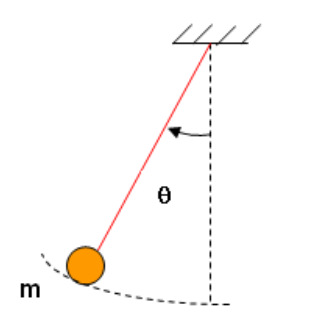
\includegraphics[clip=true,width=\columnwidth]{simple_esquema.png}
  \caption{Esquema del péndulo simple. Una partícula puntual de masa $m$ está suspendida de un punto fijo mediante un hilo de longitud $l$. El ángulo $\theta$ es el ángulo que forma el hilo con la vertical. Figura extraída de \textcolor{red}{Referencia}}
   \label{fig:simple_esquema}
\end{figure}
% https://aquinovara52.wixsite.com/misitio/post/evap3-pendulo-simple

El péndulo simple consta de una partícula puntual de masa $m$ suspendida de un punto fijo mediante un hilo de longitud $l$ (ver esquema en figura \ref{fig:simple_esquema}). La partícula se mueve en un plano y el ángulo $\theta$ que forma el hilo con la vertical se describe mediante la ecuación diferencial
\begin{equation}
  \left\{\begin{matrix}
    \theta'' = -\frac{g}{l} \sin{(\theta)} \\
    \theta(0) = \theta_0, \theta'(0) = \theta'_0
   \end{matrix}\right.
  \label{eq:pendulo_simple}
\end{equation}
donde $g$ es la aceleración de la gravedad y $\theta_0$ y $\theta'_0$ corresponden a las condiciones iniciales. Algunos parámetros importantes de la evolución del péndulo simple son el período de oscilación $\tau$ dado por
\begin{equation}
  \tau(\theta) = T_0 \left [ \sum_{n = 0}^\infty \left(  \frac{(2n)!}{2^{2n}(n!)^2} \right )^2 \sin^{2n} \left ( \frac{\theta}{2} \right )   \right ], T_0 = 2 \pi \sqrt{\frac{l}{g}},
  \label{eq:periodo_simple}
\end{equation}
la fase $\phi$ dada por
\begin{equation}
  \phi(\theta) = \tan^{-1}(\theta'/\theta)
  \label{eq:fase_simple}
\end{equation}
\textcolor{red}{ESTO ES LA FASE O EL ERROR DE FASE? LA FASE NO ES $\theta$??} y la energía por unidad de masa o amplitud $A_S$ dada por
\begin{equation}
  A^S(\theta) = 1/2 l^2 \theta'^2 - g l \cos{(\theta)}.
  \label{eq:amplitud_simple}
\end{equation}
Debido a que en el sistema actúan solo fuerzas conservativas, la amplitud $A_S$ se mantiene constante durante la evolución.

\ptitle{Ecuación vectorial del péndulo simple}

La ecuación diferencial de orden 2 de \ref{eq:pendulo_simple} se puede convertir en dos ecuaciones diferenciales de ordeen 1 mediante el cambio de variable $\vec{y_S} = (y_1, y_2) =  (\theta, \theta')$. De este modo, el problema \ref{eq:pendulo_simple} se convierte en

\begin{equation}
  \left\{\begin{matrix}
    \frac{d\vec{y_S}}{dt}  = 
    \begin{pmatrix}
    y_2 \\ -\frac{g}{l} \sin{y_1}
    \end{pmatrix}
    = \vec{f_S}(\vec{y_S},t), 
  \\
    \vec{y}_S^T(0) = (\theta_0, \theta'_0).
  \end{matrix}\right.
  \label{eq:pendulo_simple_vec}
\end{equation}

\subsection{Péndulo doble}

\ptitle{Presentar ecuaciones de la dinámica}

\begin{figure}[h]
  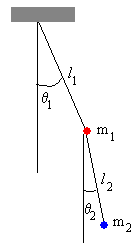
\includegraphics[clip=true,width=\columnwidth]{doble_esquema.png}
  \caption{Esquema del péndulo doble. Una partícula puntual de masa $m_1$ está suspendida de un punto fijo mediante un hilo de longitud $l_1$. El ángulo $\theta_1$ es el ángulo que forma el hilo con la vertical. Sobre esta partícula se encuentra suspendida otra de masa $m_2$ mediante un hilo de longitud $l_2$. El ángulo $\theta_2$ es el ángulo que forma este último hilo con la vertical. Figura extraída de \textcolor{red}{referencia}}
   \label{fig:doble_esquema}
\end{figure}
% http://www.sc.ehu.es/sbweb/fisica/oscilaciones/pendulo_doble/pendulo_doble.htm

El péndulo doble es un sistema más complejo que el anterior. Consta básicamente de un péndulo simple con masa $m_1$, longitud $l_1$ y ángulo $\theta_1$ sobre el que se suspende otro péndulo simple con masa $m_2$, longitud $l_2$ y ángulo $\theta_2$ (ver esquema en la figura \ref{fig:doble_esquema}). Empleando $l_1 = l_2 = 1$, $m_1 = m_2 = 1$ y $g = 10$, las ecuaciones de la evolución de los ángulos involucrados son
\begin{equation}
\left\{\begin{matrix}
  2 \theta_1'' + \theta_2'' \cos{\Delta \theta} = \theta_2'^2 \sin{\Delta \theta} - 20 \sin{(\theta_1)}, \\
  \theta_1'' \cos{\Delta \theta} + \theta_2'' = - \theta_1'^2 \sin{\Delta \theta} - 10 \sin{(\theta_2)}, \\
  \theta_1(0) = \theta_{1 0}, \theta_1'(0) = \theta_{1 0}', \\
  \theta_2(0) = \theta_{2 0}, \theta_2'(0) = \theta_{2 0}',
  \end{matrix}\right.
  \label{eq:pendulo_doble}
\end{equation}
donde $\Delta \theta = (\theta_2 - \theta_1)$.

Al igual que en el péndulo simple, la energía se conserva y la amplitud $A_D$ se mantiene constante durante la evolución. En este caso, tal amplitud está dada por
\begin{equation}
  A_D = \theta_1'^2 + \frac{1}{2} \theta_2'^2 + \theta_1' \theta_2' \cos{(\theta_2 - \theta_1)} - 20 \cos{\theta_1} - 10 \cos{\theta_2}
  \label{eq:amplitud_doble}
\end{equation}

\ptitle{Ecuación vectorial del péndulo doble}
Haciendo el cambio de variables $\vec{y_D} = (y_1, y_2, y_3, y_4) = (\theta_1, \theta_2, \theta_1', \theta_2')$, el problema \ref{eq:pendulo_doble} se convierte en

\begin{eqnarray}
  \label{eq:pendulo_doble_vec}
  \left\{\begin{matrix}
    \nonumber \frac{d\vec{y_D}}{dt} & = &
      \begin{pmatrix}
        y_3 \\
        y_4 \\
        \frac{y_4^2 \sin{\Delta} - 20 \sin{y_1} + y_3^2 \sin{\Delta} \cos{\Delta} + 10 \sin{y_2} \cos{\Delta}}{  2 - \cos^2{\Delta}  } \\
        \frac{-2 y_3^2 \sin{\Delta} - 20 \sin{y_2} - y_4^2 \sin{\Delta} \cos{\Delta} + 20 \sin{y_1} \cos{\Delta}}{  2 - \cos^2{\Delta}  }
      \end{pmatrix} \\
    \nonumber & = & \vec{f_D}(\vec{y_D},t),
    \\ \\
    \nonumber \vec{y}_S^T(0) & = &
    (\theta_{1 0}, \theta_{2 0}, \theta'_{1 0}, \theta'_{2 0})
  \end{matrix}\right.
\end{eqnarray}
  % -y_3^2 \sin{\Delta} -10 \sin{y_2} - f_3 \cos{\Delta}

% \begin{eqnarray}
%   \label{eq:pendulo_doble_vec}
%   \left\{\begin{matrix}
%     \nonumber \frac{d\vec{y_D}}{dt} & = &
%     \begin{pmatrix}
%       y_3 \\
%       y_4 \\
%       \frac{y_4^2 \sin{\Delta} - 20 \sin{y_1} + y_3^2 \sin{\Delta} \cos{\Delta} + 10 \sin{y_2} \cos{\Delta}}{  2 - \cos^2{\Delta}  } \\
%       \frac{-2 y_3^2 \sin{\Delta} - 20 \sin{y_2} - y_4^2 \sin{\Delta} \cos{\Delta} + 20 \sin{y_1} \cos{\Delta}}{  2 - \cos^2{\Delta}  }
%     \end{pmatrix}
%     = \vec{f_D}(\vec{y_D},t), \\
%     \vec{y}_S(0) =
%     \begin{pmatrix}
%       \theta_{1 0} \\ \theta_{2 0}  \\ \theta'_{1 0} \\ \theta'_{2 0}
%      \end{pmatrix},
%     \end{matrix}\right.
%    \end{matrix}\right.
% \end{eqnarray}
%   % -y_3^2 \sin{\Delta} -10 \sin{y_2} - f_3 \cos{\Delta}
% donde $\vec{y}_D^T = (y_1, y_2, y_3, y_4)$


\section{Método Numérico}

\ptitle{Para resolver estos problemas se usaron métodos numéricos. De cada método se analizó el error de fase y el error de amplitud}

Para resolver numéricamente ambos problemas de valores iniciales es necesario discretizar la variable temporal y proponer un esquema numérico que permita obtener la solución aproximada. En cuanto a lo primero, el dominio se discretizó con puntos equiespaciados $t_n = n h$ donde $n = 0, · · · , N$ y $h = 1/N$. En cuanto a lo segundo, se utilizaron en total cuatro métodos numéricos, algunos explícitos y otros implícitos. Su objetivo radica en, dado $\vec{y}_n = \vec{y}(t_n)$, aproximar $\vec{y}_{n+1}$.

Además, es necesario evaluar de alguna manera la convergencia de los métodos numéricos. Para esto se podría emplear el error respecto a la solución exacta a todo tiempo o bien evaluar el error en un tiempo específico sobre cantidades conocidas. En este trabajo se optó por lo segundo. Se evaluó para el péndulo simple el error de fase en $t = \tau$ dado por
\begin{equation}
  e_{fase}(t = \tau) = \phi_{aprox}(\tau) - \phi_{teo}(\tau) = \phi_{aprox}(\tau)
  \label{eq:simple_e_fase}
\end{equation}
pues por definición $\theta'(\tau) = 0$, y el error de amplificación en $t = \tau$ dado por
\begin{equation}
  e^S_{amp}(t = \tau) = A^S_{aprox}(\tau) - A^S_{teo}(\tau),
  \label{eq:simple_e_amp}
\end{equation}
donde $A^S_{t}$ es constante. En ambos casos, para determinar $\tau$ se empleó la expresión \ref{eq:periodo_simple} calculada con un error menor a todos los errores obtenidos en este trabajo. Mientras que para el péndulo doble se evaluó sólo el error de amplitud para todo tiempo
\begin{equation}
  e^D_{amp}(t) = A^D_{aprox}(t) - A^D_{teo}(t),
  \label{eq:doble_e_amp}
\end{equation}
donde $A^D_{t}$ también es constante en el tiempo.

Cabe preguntarse, ¿qué errores deberían obtenerse teóricamente? Se esperaría obtener el error de fase y el factor de amplificación de cada método numérico. Estos valores se encuentran tabulados y se obtienen al analizar la ecuación diferencial $y' = \lambda y$ con $\lambda$ constante con cada método en particular.

En base a lo anterior, a continuación se desarrollan los métodos numéricos utilizados, junto con el orden global de convergencia del factor de amplificación  y del error de fase. \textcolor{red}{referencia?}. Es necesario aclarar que en el caso de los métodos implícitos se utilizó el método de bisección para resolver el sistema de ecuaciones resultantes, con un error menor a todos los errores obtenidos en este trabajo.
\begin{itemize}
  \item Euler implícito (EI): este método es implícito, el factor de amplificación converge con orden $O(h^1)$ y el error de fase, con orden $O(h^2)$. Su fórmula es
  \begin{equation}
    \vec{y}_{n+1} = \vec{y}_n + h \vec{f}(\vec{y}_{n+1}, t_{n+1}) + O_{local}(h^2)
    \label{eq:Euler_implicito}
  \end{equation}

  \item Crank-Nicholson (CN): este método es implícito, el factor de amplificación es 1, por lo que se esperaría $e_{amp} = 0$ y el error de fase converge con orden $O(h^2)$. Su fórmula es
  \begin{equation}
    \vec{y}_{n+1} = \vec{y}_n + \frac{h}{2} [ \vec{f}(\vec{y}_{n+1}, t_{n+1}) + \vec{f}(\vec{y}_{n}, t_{n}) ]+ O_{local}(h^3)
    \label{eq:Crank_Nicholson}
  \end{equation}

  \item Runge Kutta 4 (RK4): este método es explícito, el factor de amplificación converge con orden $O(h^5)$ y el error de fase, con orden $O(h^4)$. Su fórmula es
  \begin{equation}
    \vec{y}_{n+1} = \vec{y}_n + \frac{1}{6} \vec{k}_1 + \frac{1}{3} (\vec{k}_2 + \vec{k}_3) + \frac{1}{6} \vec{k}_4 + O_{local}(h^5)
    \label{eq:Runge_Kutta_4}
  \end{equation}
  donde
  \[
    \left\{\begin{matrix}
      \vec{k}_1 = h \vec{f}(\vec{y}_n, t_n), \\ 
      \vec{k}_2 = h \vec{f} \left( \vec{y}_n + \frac{1}{2} \vec{k}_1 , t_n + \frac{h}{2}\right), \\
      \vec{k}_3 = h \vec{f} \left ( \vec{y}_n + \frac{1}{2} \vec{k}_2 , t_n + \frac{h}{2}  \right ), \\
      \vec{k}_4 = h \vec{f}(\vec{y}_n + \vec{k}_3, t_n + h)
    \end{matrix}\right.
  \]

  \item 2 pasos con Crank-Nicholson y uno con Leap Frog (CN + LF). Este último método es explícito, el factor de amplificación es unitario y el error de fase converge con orden $O(h^2)$. Su fórmula es
  \begin{equation}
    \vec{y}_{n+1} = \vec{y}_{n-1} + 2 h \vec{f}(\vec{y}_n, t_n) + O_{local}(h^3)
    \label{eq:Leap_Frog}
  \end{equation}
  El objetivo de combinar ambos métodos de esta forma en particular es que los errores de fase se compensan para dar un orden de convergencia mayor, de al menos $O(h^3)$. \textcolor{red}{Está bien esta afirmación? Sí}. Aún más, el factor de amplificación se mantiene unitario.


\end{itemize}

\ptitle{Resumen de lo que se hará. Qué se resuelve con qué}
Se resolvió el péndulo simple con los cuatro esquemas numéricos mencionados. Se evaluó el orden de convergencia de $e_{fase}$ y $e_{amp}$ y se comparó con los valores teóricos. Además, se resolvió el péndulo doble con \textcolor{red}{COMPLETAR}


\section{Resultados y discusión}

\subsection{Péndulo simple}

Se resolvió el péndulo simple con los cuatro esquemas numéricos mencionados para las condiciones iniciales $\theta_0 = \pi/2$ y $\theta'_0 = 0$ con $h = 0.1$. La evolución de $\theta(t)$ se grafica en la figura \ref{fig:sol_aprox}. Por un lado, se observa que la amplitud de variación de $\theta(t)$, relacionada con la amplitud $A^S$, no es constante para algunos métodos, siendo el caso más notable el de Euler implícito. Por otro lado, para algunos méotodos se observa un cambio en la fase, es decir, el tiempo en el que $\theta(t)$ alcanza su valor máximo no es idéntico para todos. Esto implica que existe un error de fase, como se esperaría a partir del análisis realizado en la sección anterior.


\begin{figure}[h]
  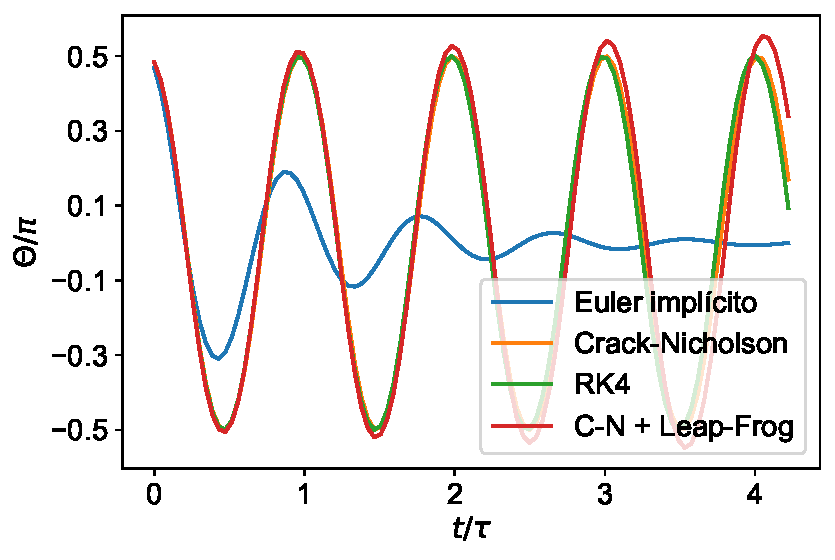
\includegraphics[clip=true,width=\columnwidth]{sol_aprox.pdf}
  \caption{Evolución de $\theta(t)$ para los cuatro esquemas numéricos para las condiciones iniciales $\theta_0 = \pi/2$ y $\theta'_0 = 0$ con $h = 0.1$. Ambos ejes se encuentran normalizados: el eje vertical por $\pi$ y el horizontal por el período $\tau$.}
   \label{fig:sol_aprox}
\end{figure}

Para todos los métodos se calculó $e_{fase}$ para distintos valores de $h$ y se determinó el orden de convergencia. 
\begin{itemize}
  \item La dependencia del error con el tamaño de la discretización para todos los esquemas se grafica en la figura \ref{fig:error_fase_simple_pi2} en escala log-log. \item En todos los casos se obtuvo un comportamiento lineal a partir de un valor de $h$ suficientemente pequeño. En base a esto, se ajustó una recta para cada caso, obteniendo el orden de convergencia de cada método.
  \item Los resultados se resumen en la tabla \textcolor{red}{ref tabla}
  \item Análisis de resultados
\end{itemize}




Análogamente, se calculó $e_{amp}$ en función de $h$ y se determinó el orden de convergencia. Tal dependencia se grafica en la figura \ref{fig:error_amplitud_simple_pi2}. A diferencia del caso anterior, si bien se observa un comportamiento lineal, para $h$ suficientemente pequeño, los métodos RK4 y CN alcanzan un valor constante, \textcolor{red}{lo cual puede deberse a errores de punto flotante? En el caso de ángulo pequeño alcanza errores menores}. De todos modos, se realiza un ajuste lineal sobre la zona con compotamiento lineal. La pendiente del ajuste corresponde al orden de convergencia del error y se resumen en la tabla \textcolor{red}{tabla}.
\begin{itemize}
  \item Análisis de la tabla
\end{itemize}



\begin{itemize}
  \item En ambos casos anteriores no se obtuvieron los valores teóricos. Esto pudo deberse a que los órdenes de convergencia mencionados se calculan en base a un problema lineal $y' = \lambda y$. En el caso de la ecuación de movimiento, el problema es no lineal y por lo tanto no se puede esperar que los órdenes de convergencia sean los mismos. Sin embargo, sí se esperaría obtener los mismos valores para $\tita \rightarrow 0$, debido a que en este caso la ecuación de movimiento se reduce a un problema lineal.
  \item En base a esto, se calculó la dependencia de $e_{fase}$ y $e_{amp}$ en función de $h$ para $\theta = 0.01$. Los resultados se grafican en las figuras \ref{fig:error_fase_simple_angulo_bajo} y \ref{fig:error_amplitud_simple_angulo_bajo}, respectivamente. 
\end{itemize}

\onecolumngrid

% Please add the following required packages to your document preamble:
% \usepackage{multirow}
\begin{table}[]
  \begin{tabular}{|c|llllll|}
  \hline
  \multirow{3}{*}{Método} &
    \multicolumn{6}{c|}{Orden de convergencia de} \\ \cline{2-7} 
   &
    \multicolumn{3}{c|}{$e_{fase}$} &
    \multicolumn{3}{c|}{$e_{amp}$} \\ \cline{2-7} 
   &
    \multicolumn{1}{c|}{teórico} &
    \multicolumn{1}{c|}{con $\theta_0 = \pi/2$} &
    \multicolumn{1}{c|}{con $\theta_0 = 0.01$} &
    \multicolumn{1}{c|}{teórico} &
    \multicolumn{1}{c|}{con $\theta_0 = \pi/2$} &
    \multicolumn{1}{c|}{con $\theta_0 = 0.01$} \\ \hline
  EI &
    \multicolumn{1}{l|}{2} &
    \multicolumn{1}{l|}{$0.91 \pm 0.03$} &
    \multicolumn{1}{l|}{$1.97 \pm 0.03$} &
    \multicolumn{1}{l|}{1} &
    \multicolumn{1}{l|}{$0.94 \pm 0.02$} &
    $0.91 \pm 0.03$ \\ \hline
  CN &
    \multicolumn{1}{l|}{2} &
    \multicolumn{1}{l|}{$1.96 \pm 0.02$} &
    \multicolumn{1}{l|}{$1.93 \pm 0.04$} &
    \multicolumn{1}{l|}{0} &
    \multicolumn{1}{l|}{$5.79 \pm 0.09$} &
    0 \\ \hline
  RK4 &
    \multicolumn{1}{l|}{4} &
    \multicolumn{1}{l|}{$3.92 \pm 0.02$} &
    \multicolumn{1}{l|}{$4.02 \pm 0.02$} &
    \multicolumn{1}{l|}{5} &
    \multicolumn{1}{l|}{$4.87 \pm 0.04$} &
    $4.94 \pm 0.03$ \\ \hline
  CN + LF &
    \multicolumn{1}{l|}{3} &
    \multicolumn{1}{l|}{$1.86 \pm 0.05$} &
    \multicolumn{1}{l|}{$1.96 \pm 0.02$} &
    \multicolumn{1}{l|}{0} &
    \multicolumn{1}{l|}{$2.96 \pm 0.05$} &
    $3.010 \pm 0.005$ \\ \hline
  \end{tabular}
  \caption{\label{tabla:simple_errores} Orden de convergencial del error de fase $e_{fase}$ y del error de amplitud $e_{amp}$ para los cuatro esquemas numéricos bajo las condiciones iniciales $\theta'_0 = 0$ y distintos valores de $\theta_0$. 'EI': Euler implícito, 'C-N': Crank-Nicholson, 'RK4': Runge-Kutta 4 y 'C-N + L-F': dos pasos con Crank Nicholson y uno con Leap-Frog.}
  \end{table}

\textcolor{red}{En el problema lineal el error de fase cometido en cada paso no depende del paso, entonces tiene sentido hacer sumar y restar errores con CN y LF. Pero en el problema no lineal el error de fase depende del punto en el que estoy mirando y por lo tanto no se cancelan. Aún así, el orden aumenta a menor tita inicial}

\textcolor{red}{En CN y LF el error de amplitud debería ser cero. No lo es, pero aún así cuando bajo tita inicial aumenta el orden de convergencia. Mencionar que no pude disminuir mucho más tita inicial por un problema de representación (sólo puedo usar 16 dígitos en Octave)}

% \begin{figure}[h]
%   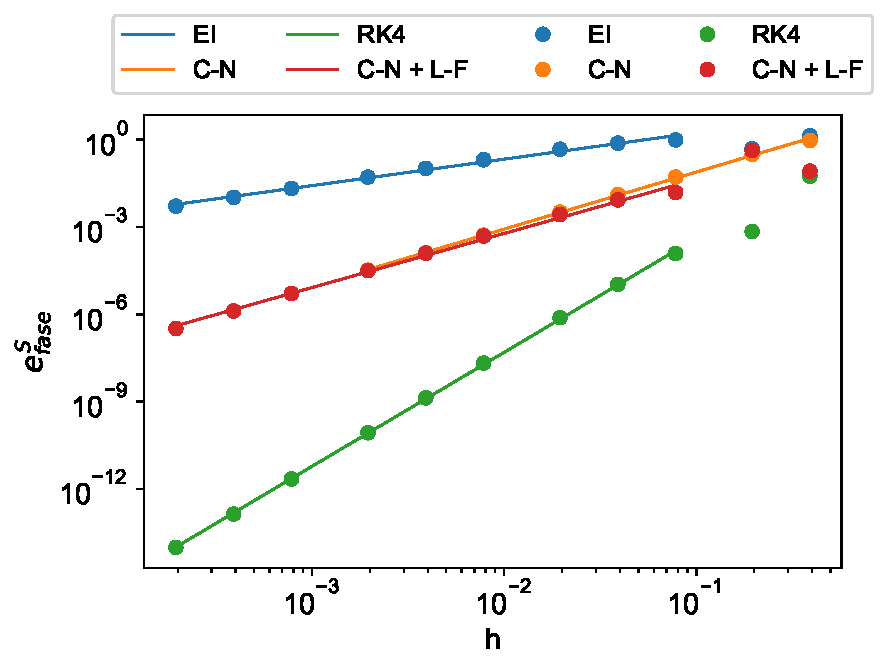
\includegraphics[clip=true,width=\columnwidth]{error_fase_simple_pi2.pdf}
%   \caption{Error de fase $e_{fase}$ para los cuatro esquemas numéricos en función del tamaño de la discretización $h$ bajo las condiciones iniciales $\theta_0 = \pi/2$ y $\theta'_0 = 0$. Los puntos corresponden a los valores calculados y las líneas a los ajustes lineales. 'EI': Euler implícito, 'C-N': Crank-Nicholson, 'RK4': Runge-Kutta 4 y 'C-N + L-F': 2 pasos con Crank Nicholson y uno con Leap-Frog.}
%    \label{fig:error_fase_simple_pi2}
% \end{figure}
% % FASE:
% % Orden de convergencia Euler implícito:  0.9094202564952926 +/- 0.03070835705396524, o sea, $0.91 \pm 0.03$
% % Orden de convergencia Crack-Nicholson:  1.9609514818114762 +/- 0.019260309080823608, o sea, $1.96 \pm 0.02$
% % Orden de convergencia RK4:  3.9163907216640714 +/- 0.02044736620447468, o sea, $3.92 \pm 0.02$
% % Orden de convergencia C-N + Leap-Frog:  1.8573616277295897 +/- 0.04875131838369911, o sea, $1.86 \pm 0.05$


% \begin{figure}[h]
%   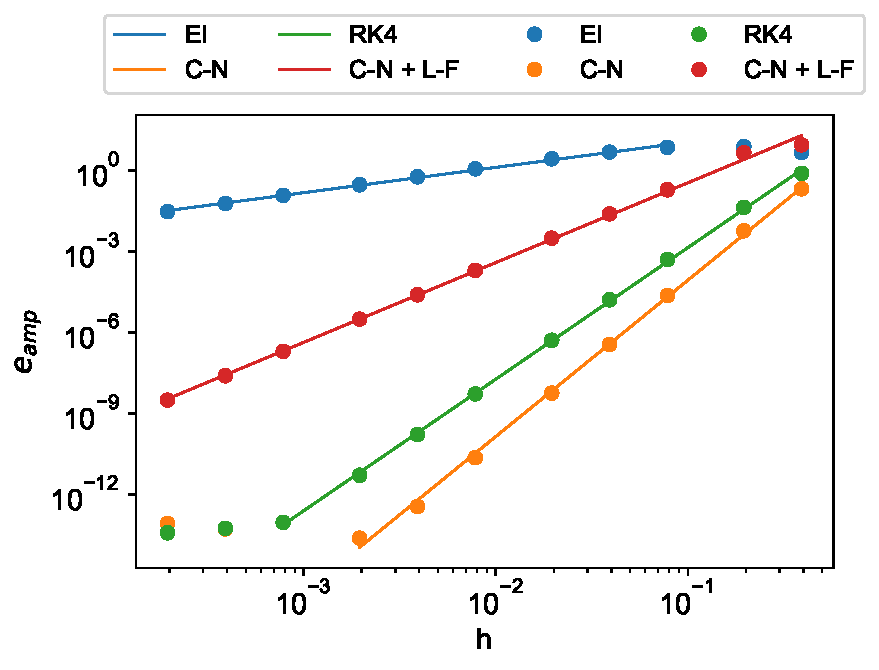
\includegraphics[clip=true,width=\columnwidth]{error_amplitud_simple_pi2.pdf}
%   \caption{Error de amplitud $e_{amp}$ para los cuatro esquemas numéricos en función del tamaño de la discretización $h$ bajo las condiciones iniciales $\theta_0 = \pi/2$. \textcolor{red}{Los puntos...}}
%    \label{fig:error_amplitud_simple_pi2}
% \end{figure}

% % AMPLITUD:
% % Orden de convergencia Euler implícito:  0.9372575985568138 +/- 0.01902503308713794, o sea, $0.94 \pm 0.02$
% % Orden de convergencia Crack-Nicholson:  5.790183279314054 +/- 0.09070012637078931, o sea, $5.79 \pm 0.09$
% % Orden de convergencia RK4:  4.872347720305063 +/- 0.03460069824650806, o sea, $4.87 \pm 0.04$
% % Orden de convergencia C-N + Leap-Frog:  2.9552896088114005 +/- 0.04216313986505771, o sea, $2.96 \pm 0.05%



% \begin{figure}[h]
%   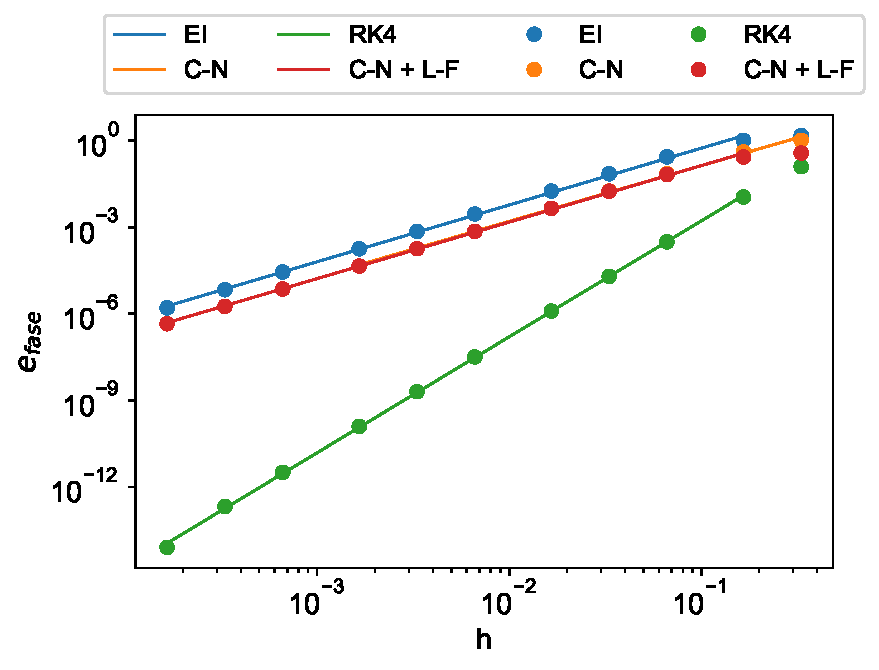
\includegraphics[clip=true,width=\columnwidth]{error_fase_simple_angulo_bajo.pdf}
%   \caption{\textcolor{blue}{(b) Error de amplitud para los 4 métodos para tita inicial de 10e-4}}
%    \label{fig:error_fase_simple_angulo_bajo}
% \end{figure}
% % FASE:
% % Orden de convergencia Euler implícito:  1.969515531340741 +/- 0.02352945286109731, o sea, $1.97 \pm 0.03$
% % Orden de convergencia Crack-Nicholson:  1.9315725179531302 +/- 0.031743969584564165, o sea, $1.93 \pm 0.04$
% % Orden de convergencia RK4:  4.020308658595079 +/- 0.020460933506094077, o sea, $4.02 \pm 0.02$
% % Orden de convergencia C-N + Leap-Frog:  1.9591911569629437 +/- 0.019303222788158225, o sea, $1.96 \pm 0.02$


% \begin{figure}[h]
%   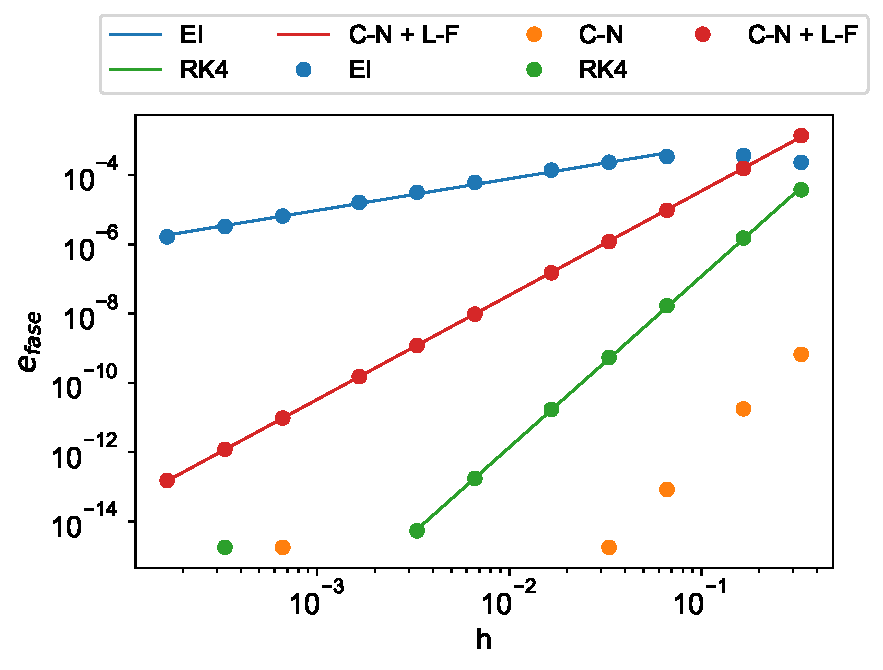
\includegraphics[clip=true,width=\columnwidth]{error_amplitud_simple_angulo_bajo.pdf}
%   \caption{\textcolor{blue}{(a) Error de fase para los 4 métodos para tita inicial de 10e-4}}
%    \label{fig:error_amplitud_simple_angulo_bajo}
% \end{figure}
% % AMPLITUD:
% % Orden de convergencia Euler implícito:  0.9125871407963045 +/- 0.023038374694042806, o sea, $0.91 \pm 0.03$
% % Orden de convergencia RK4:  4.940148423340664 +/- 0.023908301779203472, o sea, $4.94 \pm 0.03$
% % Orden de convergencia C-N + Leap-Frog:  3.0099767594644535 +/- 0.004694372715781479, o sea, $3.010 +/- 0.005$
% % CN tiene error cero creo



\begin{figure}
  \centering
  \begin{subfigure}[b]{0.45\textwidth}
      \centering
      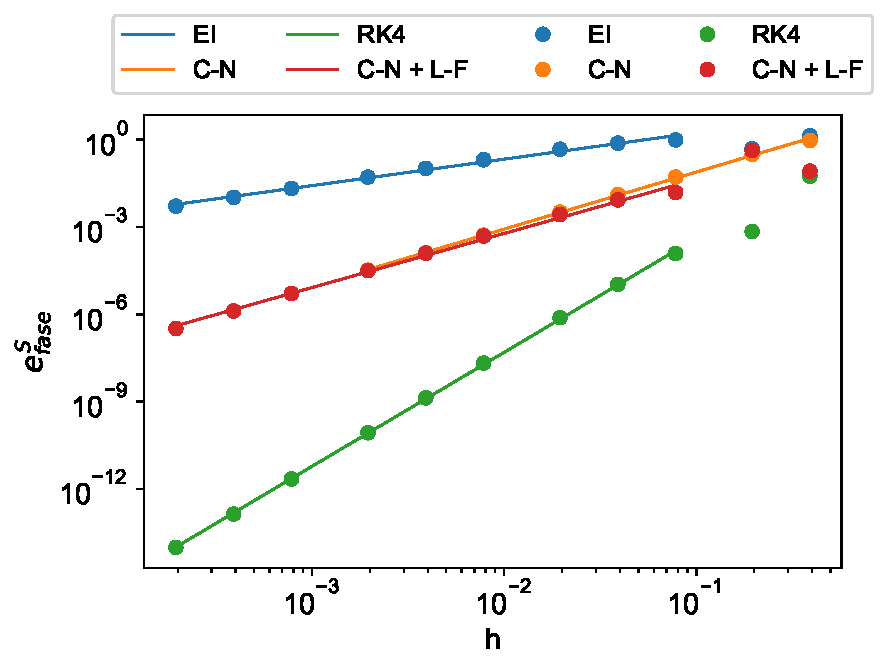
\includegraphics[width=\textwidth]{error_fase_simple_pi2.pdf}
      \caption{\label{fig:error_fase_simple_pi2}}
  \end{subfigure}
  \hfill
  \begin{subfigure}[b]{0.45\textwidth}
      \centering
      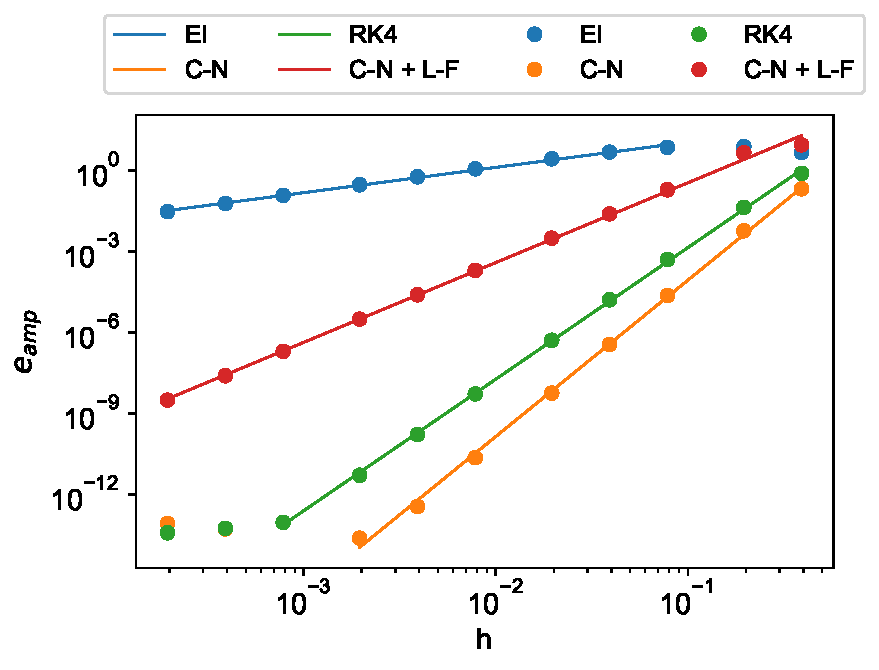
\includegraphics[width=\textwidth]{error_amplitud_simple_pi2.pdf}
      \caption{\label{fig:error_amplitud_simple_pi2}}
  \end{subfigure}
  \hfill
  \begin{subfigure}[b]{0.45\textwidth}
      \centering
      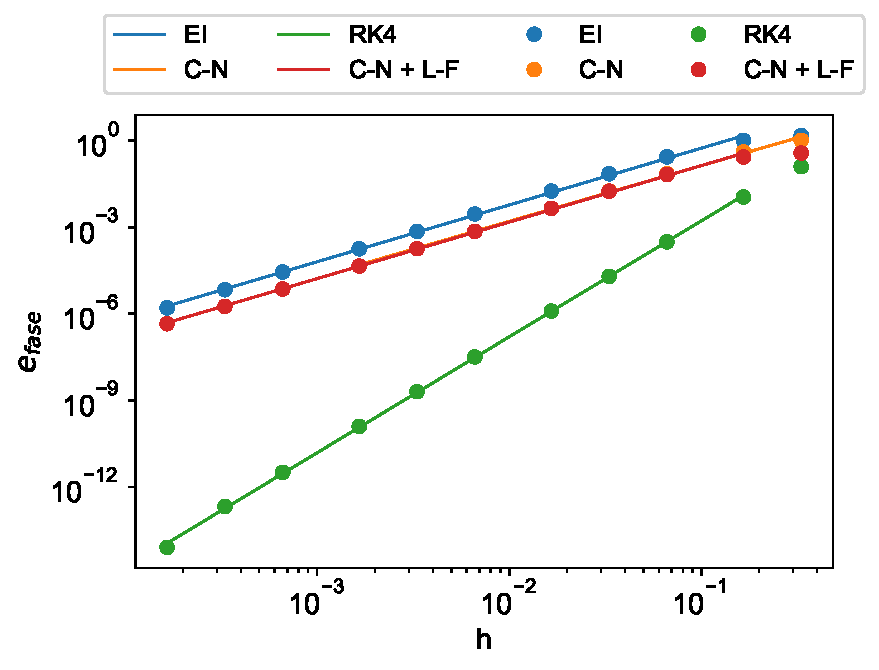
\includegraphics[width=\textwidth]{error_fase_simple_angulo_bajo.pdf}
      \caption{\label{fig:error_fase_simple_angulo_bajo}}
  \end{subfigure}
  \hfill
  \begin{subfigure}[b]{0.45\textwidth}
      \centering
      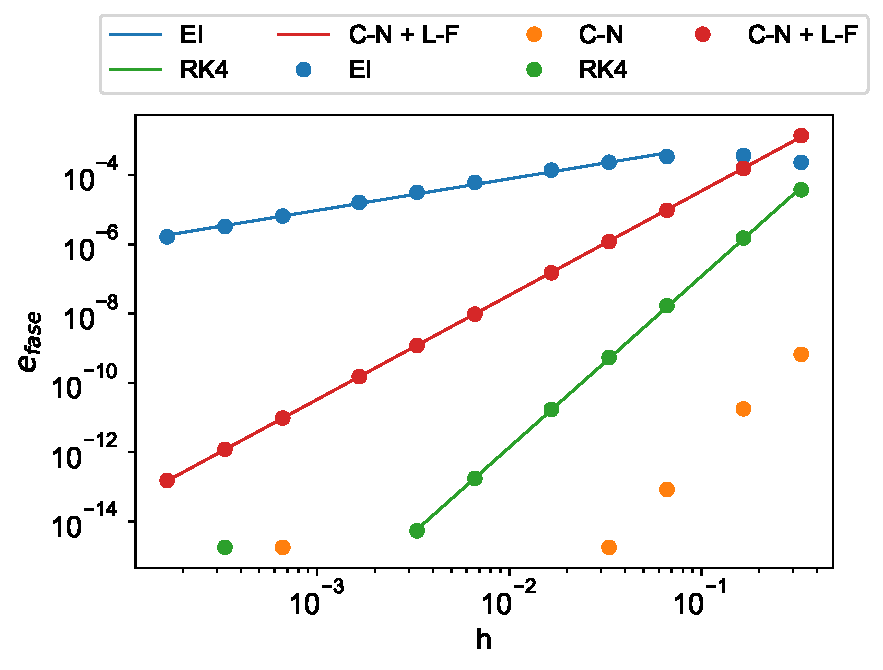
\includegraphics[width=\textwidth]{error_amplitud_simple_angulo_bajo.pdf}
      \caption{\label{fig:error_amplitud_simple_angulo_bajo}}
  \end{subfigure}
     \caption{Error de fase $e_{fase}$ y error de amplitud $e_{amp}$ en función del tamaño de la discretización $h$ para los cuatro esquemas numéricos bajo las condiciones iniciales \ref{fig:error_fase_simple_pi2} y \ref{fig:error_amplitud_simple_pi2}, $\theta_0 = \pi/2$ y $\theta'_0 = 0$, \ref{fig:error_fase_simple_angulo_bajo} y \ref{fig:error_amplitud_simple_angulo_bajo}, $\theta_0 = 0.01$ y $\theta'_0 = 0$ . Los puntos corresponden a los valores calculados y las líneas a los ajustes lineales. 'EI': Euler implícito, 'C-N': Crank-Nicholson, 'RK4': Runge-Kutta 4 y 'C-N + L-F': dos pasos con Crank Nicholson y uno con Leap-Frog.}
     \label{fig:simple_error_vs_h}
\end{figure}




\twocolumngrid






\subsection{Péndulo doble}

\begin{figure}[h]
  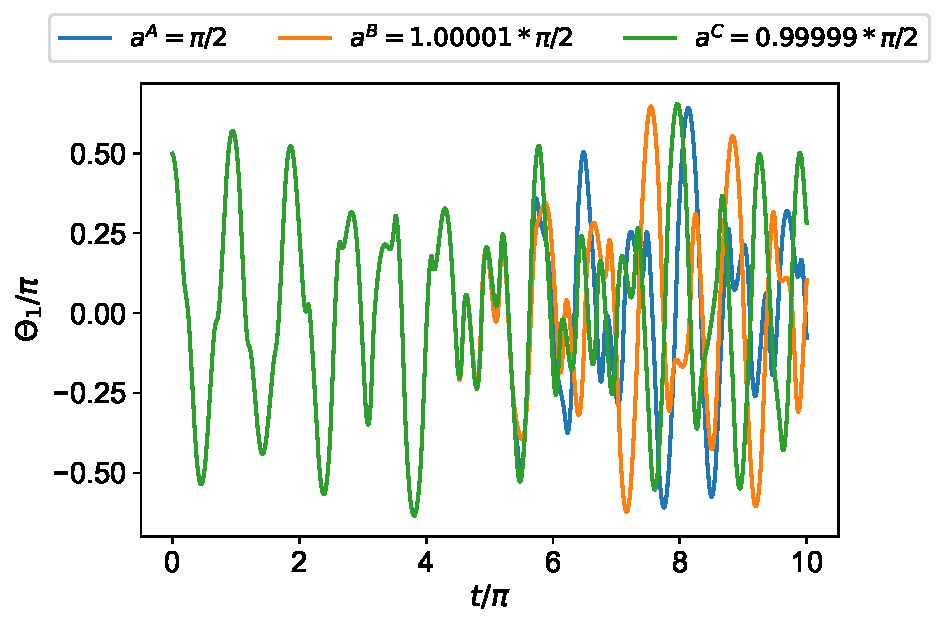
\includegraphics[clip=true,width=\columnwidth]{doble_3CI.pdf}
  \caption{Evolución de $\theta_1(t)$ para los cuatro esquemas numéricos para las condiciones iniciales $\theta_{1 0} = \pi/2$, $\theta_{2 0} = a$ y $\theta'_{1 0} = \theta'_{2 0} = 0$ con $h = \pi/100$. Ambos ejes se encuentran normalizados por $\pi$.}
   \label{fig:doble_3CI}
\end{figure}


\begin{figure}[h]
  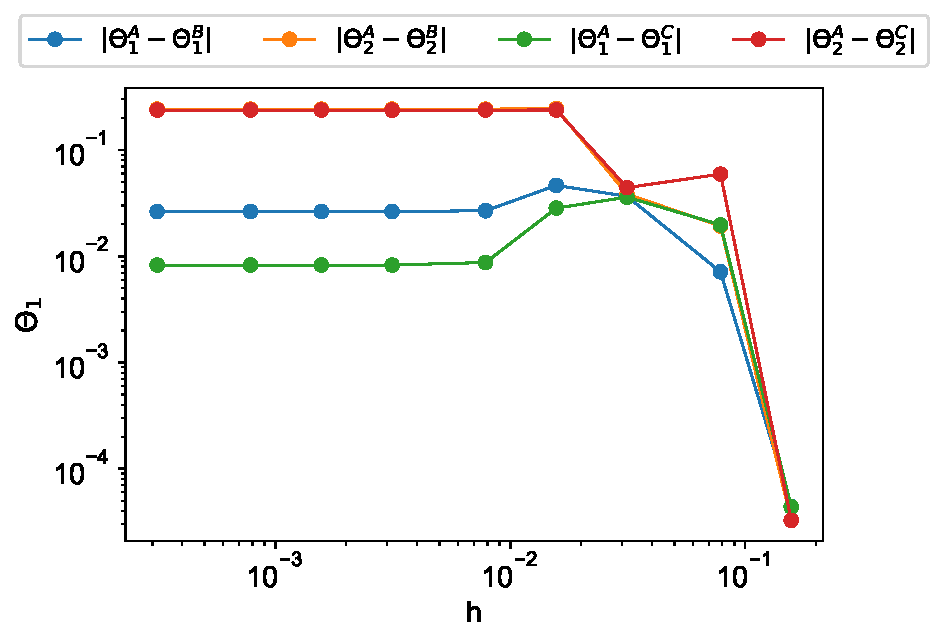
\includegraphics[clip=true,width=\columnwidth]{doble_3CI_difs.pdf}
  \caption{\textcolor{blue}{Diferencias entre las soluciones numéricas a tiempo fijo en función de h}}
   \label{fig:doble_3CI_difs}
\end{figure}

\begin{figure}[h]
  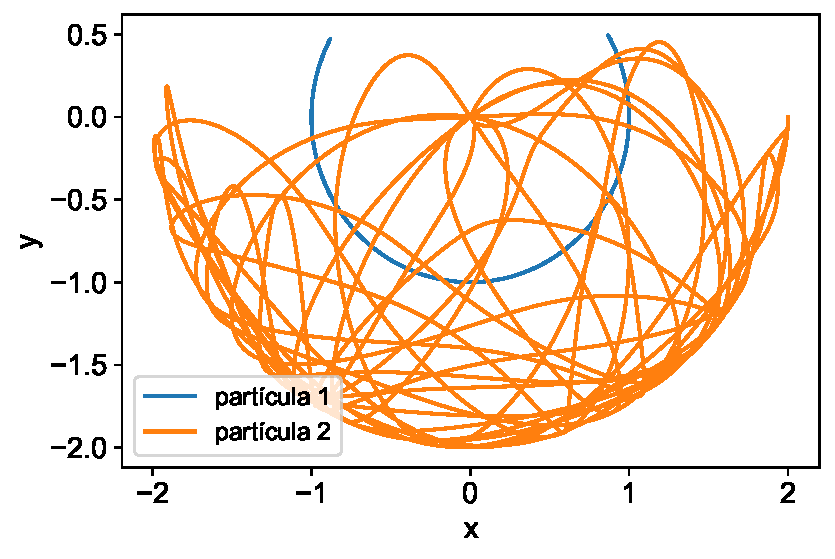
\includegraphics[clip=true,width=\columnwidth]{doble_1CI_trayectorias.pdf}
  \caption{\textcolor{blue}{Trayectorias de las 1 condiciones iniciales}}
   \label{fig:doble_1CI_trayectorias}
\end{figure}

\begin{figure}[h]
  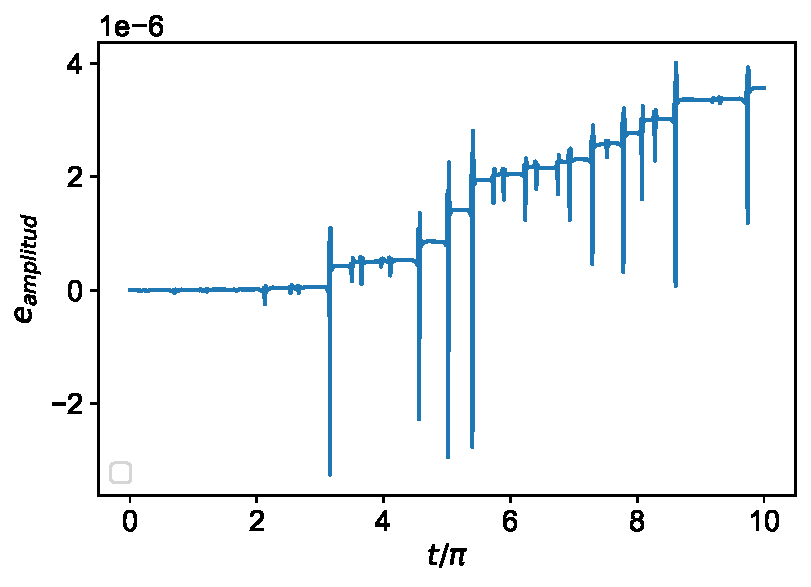
\includegraphics[clip=true,width=\columnwidth]{doble_error_amplitud.pdf}
  \caption{\textcolor{blue}{Error de amplitud para todo tiempo}}
   \label{fig:doble_error_amplitud.pdf}
\end{figure}

\begin{figure}[h]
  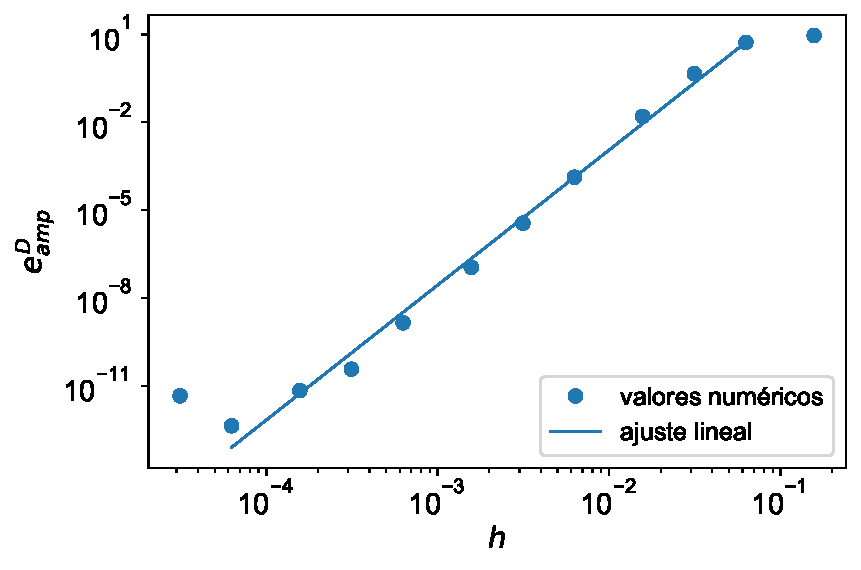
\includegraphics[clip=true,width=\columnwidth]{doble_orden_error_amplitud.pdf}
  \caption{\textcolor{blue}{Orden del error de amplitud}}
   \label{fig:doble_orden_error_amplitud}
\end{figure}


\section{Conclusión}




\bibliography{Chehade_guia1.bib}

\end{document}





